% Chapter 3
\chapter{Method and Implementation}
\label{chap:Chapter3}

This chapter details the methodology employed to tackle the problem, providing an overview of the technologies utilized and the implementation process. 

It consists of two sections: the first describes the method's design and proposed solutions, while the second covers the proof of concept, including implementation and optimization in a live environment.

\section{Method}
This section describes the methodological foundation of the project. 
It begins by presenting the technologies used and continues with an outline of three distinct solution strategies to the problem. 

Each approach is described through its pipeline and architectural design, offering a comparative view of possible solutions.

\subsection{Technological Overview}

The solution will be developed and implemented using the Python programming language, version 3.10.12. 
The following libraries are expected to be used throughout the development of the project:

\begin{itemize}
    \item \textbf{scikit-learn} (version 1.6.1): This library will be used for building machine learning models, including the Random Forest model. It provides necessary functionalities for model training, testing, and performance evaluation.
    
    \item \textbf{pandas} (version 2.2.3): Pandas will be used for data manipulation and analysis, particularly for handling, processing, and cleaning the alert datasets. It provides efficient data structures for handling large amounts of structured data.

    \item \textbf{fastapi} (version 0.115.11): FastAPI will be used to create the necessary APIs for data flow between the components. It will expose endpoints for the system, allowing real-time predictions and feedback from analysts to be communicated between the machine learning models and the IBM SOAR interface.

    \item \textbf{matplotlib} (version 3.10.1): Matplotlib will be used to generate plots and graphs, particularly for data exploration, visualizing model performance, and evaluating results. It will assist in identifying patterns in the data and understanding how well the model is classifying the security alerts.

    \item \textbf{SentenceTransformer} (likely needed): SentenceTransformer will be used for text vectorization, particularly for converting textual data such as alert descriptions and analyst comments into numerical embeddings. These embeddings will be used as inputs to machine learning models for better understanding and classification of textual data.

\end{itemize}


\subsection{Problem-Solving Approaches}
This subsection analyzes three distinct approaches to tackling the identified problem. 
It outlines the specific methodologies employed for each approach, detailing the pipeline process involved and the architectural framework that supports its implementation.

\paragraph{Pipeline}

Figure~\ref{fig:general_solution_pipeline} represents the general data processing pipeline for all solutions, illustrating the flow of data through various stages before it reaches the analyst. 

The pipeline is designed to handle security alerts from multiple sources, process the data, and present the predictions to the analyst.

\begin{figure}[h!]
    \centering
    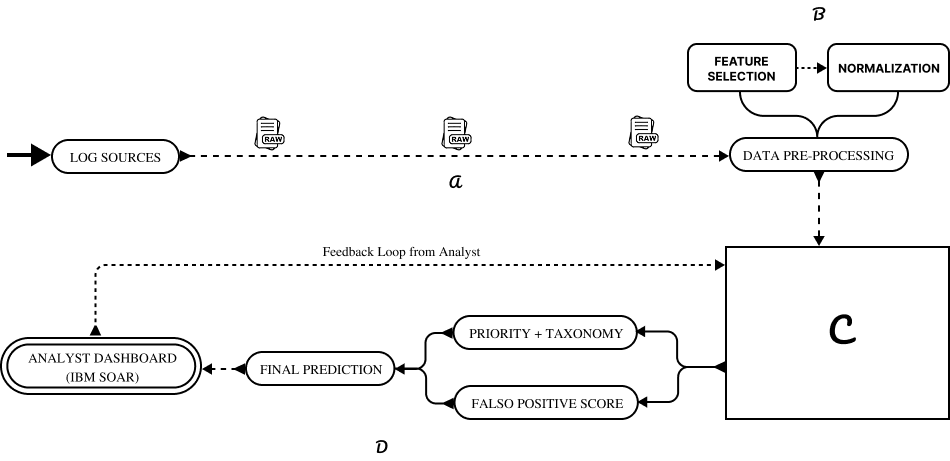
\includegraphics[width=\textwidth]{ch3/assets/general_solution_pipeline.png}
    \caption{General Pipeline for all Three Solutions}
    \label{fig:general_solution_pipeline}
\end{figure}

This pipeline remains largely the same across all solutions, with the exception of section \texttt{C}, where the machine learning model varies depending on the solution. 
While the overall structure of the pipeline is consistent, the type of model used in section \texttt{C} determines the specific prediction process and outputs.

The described pipeline includes several key stages:
\begin{itemize}
    \item \textbf{Raw security alert data ingestion:} In section \texttt{A}, alert data is collected from various log sources, such as SIEM systems, IDS, and firewalls. This data typically contains a wide range of information, including alert descriptions, timestamps, and metadata. In this section, the data is prepared for processing by standardizing the format across different sources.
    \item \textbf{Data pre-processing:} In section \texttt{B}, the collected data undergoes a series of cleaning and normalization procedures. This stage includes feature extraction, where relevant information from the raw data is transformed into structured, usable features.
    \item \textbf{Machine Learning Model (specific to each solution):} Section \texttt{C} involves feeding the pre-processed data into the machine learning model. The core of this section differs depending on the solution.
    \item \textbf{Final predictions for the analyst dashboard:} After the predictions are generated in section \texttt{C}, the results are passed on to the IBM SOAR dashboard, section \texttt{D}. This dashboard presents the predictions to the analyst, who can review the outputs, including taxonomy, priority, false positive status, and confidence score. The analyst can provide feedback on these predictions, which is sent back into the system to refine future predictions, contributing to the model's long-term accuracy and adaptability.
\end{itemize}

This pipeline was designed to be modular and flexible, allowing for easy integration with existing systems and the ability to adapt to evolving security threats.

\subsubsection{Random Forest with Reinforcement Learning Feedback Loop}

The first solution proposed in this study is a two-layered machine learning system that integrates a Random Forest model with a Reinforcement Learning feedback loop. 

This solution addresses the problem using a pre-trained RF model on historical data combined with an RL model that refines predictions based on analyst feedback.
This integration of \underline{RF with RL} contributes to the model's adaptability, making it highly responsive to new threats.

\paragraph{Design} 

The RF model serves as the decision-making core, trained on a historical dataset of security alerts to classify incoming alerts by taxonomy and priority—\hyperref[objective3]{Objective 3}.

While the RF model provides strong initial predictions, it struggles to adapt to new attack vectors not represented in its training data. 
To address this, the RL model enhances the predictions made by the RF model and evaluates alerts as false positives or true positives, using feedback from security analysts.

The \underline{implementation complexity} of this solution is considered \underline{moderate}, as it does not involve highly intricate algorithms or architectures. 
However, the necessity to implement and integrate two distinct models—a RF for initial predictions and a RL model for feedback-driven refinement—adds an additional layer of complexity. 

Key features of this solution include:
\begin{itemize}
    \item The RL model adjusts its parameters through a continuous feedback loop, improving classification and generating confidence scores.
    \item This dynamic learning process ensures the system is able to handle both \underline{\texttt{cold start}} issues effectively (thanks to the pre-trained RF model) and false positives in real-time.
    \item The system's \underline{adaptability} to new threats is \underline{high via the RL model} and helps manage false positives by learning patterns of false positives or true positives, refining its algorithms, and potentially reducing analysts' workloads.
    \item Designed to efficiently manage and analyze real-time alerts generated from a diverse range of log sources—\hyperref[objective4]{Objective 4}.
\end{itemize}

The \underline{interpretability} of this solution is considered \underline{moderate} due to the significant role played by AI in its decision-making processes. 
The RF model, being a supervised learning algorithm, provides a level of transparency as its outputs can be traced back to the quality and features of the historical dataset used for training. 

However, integrating RL complicates interpretability. RL's iterative feedback and rewards lead to less transparent reasoning, making analyzing and communicating insights challenging.

Integrating this solution with \underline{IBM SOAR} is relatively \underline{easy and straightforward}. 
By relying on the API endpoints provided by this solution, IBM SOAR can seamlessly communicate with the solution platform.
This is vital for enhancing the overall effectiveness of the solution—\hyperref[objective5]{Objective 5}. 

IBM SOAR provides customization of dashboards presented to analysts, enabling:

\begin{itemize}
    \item Creation of custom fields where analysts can view the solution's outputs and mark them as correct or incorrect.
    \item Feedback from analysts, which is crucial for the RL model to learn from mistakes and improve over time.
\end{itemize}

This feedback loop supports continuous refinement and enhances accuracy for future predictions. 
Overall, this strategy leverages the strengths of supervised and reinforcement learning to create a robust solution for security alert triage. 
It enhances operational efficiency and threat response capabilities by:

\begin{itemize}
    \item Minimizing false positives through continuous improvement.
    \item Allowing integration with IBM SOAR to evaluate and test the solution's effectiveness in categorizing alerts and minimizing false positives—\hyperref[objective6]{Objective 6}.
\end{itemize}

\paragraph{Pipeline} 

The illustration in Figure~\ref{fig:solution1_c} corresponds to section \texttt{C} of the general pipeline in Figure~\ref{fig:general_solution_pipeline}. 

\begin{figure}[h!]
    \centering
    
\includegraphics[width=0.5\textwidth]{ch3/assets/solution1_C.png}
    \caption{Part C of the General Pipeline for the Random Forest with Reinforcement Learning Feedback Loop Solution}
    \label{fig:solution1_c}
\end{figure}

This figure provides a detailed representation of the machine learning model's specific implementation for this solution. 

It elaborates on the processes and components that occur within section \texttt{C}, as outlined in the general pipeline, showcasing the unique aspects of this solution's approach to data processing and prediction generation.

\subsubsection{End-to-End Deep Learning Classifier with Feature Fusion}
The second solution in this study employs a deep neural network (DNN) model trained end-to-end on labeled security alert data, based on historical alerts dataset—\hyperref[objective3]{Objective 3}. 

Unlike solution one, which uses a pre-trained RF model, this approach processes raw SIEM logs, analyst comments, and metadata through the DNN's attention layers to automatically extract features and classify data, eliminating the need for manual feature engineering.

While solution one adapts to new threats with a reinforcement learning feedback loop, solution two relies solely on the DNN model, necessitating training on a comprehensive dataset before deployment. 
The DNN excels in complex feature extraction environments but requires periodic retraining based on analyst feedback.

\paragraph{Design}

In this solution, the \underline{DNN model} processes raw security alert data directly, leveraging attention mechanisms to identify and prioritize critical features like alert descriptions, origins, and metadata. 

The attention layers enhance the model's ability to focus on relevant patterns, improving classification accuracy and adaptability. 

By automating feature extraction, this approach streamlines the pipeline, reducing dependency on domain-specific preprocessing techniques.

Key aspects of this solution are:
\begin{itemize}
    \item The DNN model takes in raw security alert data, which is vectorized, and outputs predictions on alert taxonomy, priority, false positive status, and confidence score.
    \item The DNN model's \underline{adaptability} is \underline{moderate} and depends on the training data's quality and diversity. Once trained, it performs well on known data but is less responsive to new attack patterns unless retrained with fresh data.
    \item Solution two faces challenges with cold start problems, as the DNN model requires a substantial amount of labeled training data before it can begin making accurate predictions. Unlike solution one, which benefits from the pre-trained RF model, this solution requires extensive training before it can function effectively.
    \item Engineered to effectively process and evaluate real-time alerts originating from a wide variety of log sources—\hyperref[objective4]{Objective 4}.
\end{itemize}

The \underline{implementation complexity} of solution two is considered \underline{high} due to the extensive computational resources required to train the DNN model. 
Training a deep neural network, especially one that handles raw alert data with attention mechanisms, demands significant time and resources, making it more complex to implement.

The \underline{interpretability} of the solution is \underline{low}, primarily because the DNN model operates as a "black box". 
While it offers powerful predictions, the model's inner workings are difficult to explain, particularly when attention layers are involved, making it harder to interpret why certain predictions were made.

This solution integrates with IBM SOAR for real-time feedback and performance evaluation—\hyperref[objective5]{Objective 5}, allowing analysts to review predictions and provide feedback, which is subsequently used for periodic retraining to assess and validate the solution's capability in classifying alerts and reducing the occurrence of false positives—\hyperref[objective6]{Objective 6}.

\subsubsection{Rule-Augmented Decision Tree with Feedback Aggregation}

The third solution proposed in this study integrates static expert rules with a lightweight \underline{\gls{DTC}}. 
This hybrid system uses a rule engine to pre-filter known benign or critical alert patterns before passing any unknown or ambiguous cases to the \underline{\gls{DTM}}. 

The rules provide initial filtering for quick decisions on clear alerts. For complex cases, the DTC predicts based on available data. 
Feedback is reviewed in batches, enabling periodic updates to the rule base and retraining of the decision tree.

\paragraph{Design}

This solution combines the benefits of domain-specific rules with machine learning.
It starts with a rule engine that quickly processes alerts based on known patterns, tagging them as benign or critical and minimizing the need for further analysis. 
This approach is efficient in environments with well-defined, static patterns. 
This solution will be designed to ingest data from a variety of log sources, including SIEM systems and other security tools—\hyperref[objective4]{Objective 4}.

The rule engine will preprocess and filter alerts from these sources, leveraging predefined rules to handle known patterns efficiently, while less adaptive, predefined rules to filter known benign patterns, ensuring a baseline reduction in false positives. 

For alerts that don't fit predefined rules, the DTC classifies them using features from raw data, allowing the system to manage both known and unknown patterns while balancing interpretability and accuracy. 

The DTC works with a clean, segmented dataset to differentiate between alerts that match known patterns and those requiring further analysis—\hyperref[objective3]{Objective 3}.

Key features of this solution include:
\begin{itemize}
    \item The rule engine filters known benign or critical patterns before passing uncertain alerts to the DTC. This approach reduces the overall processing time and helps prioritize more ambiguous cases.
    \item \underline{Feedback} is logged and applied asynchronously, meaning that the system doesn't update in real-time. Instead, the rule base is updated, and the decision tree is retrained on a \underline{periodic basis (e.g., weekly)}. This ensures that the system evolves over time but does not immediately adjust to new threats in real-time.
    \item The system's ability to \underline{handle new and evolving threats} is \underline{low}, as it depends on manually updating the rule base to address new threats.
    \item \underline{\textit{Cold start}} handling is excellent because the rules-based filtering system can operate immediately without requiring training, and the DTC is lightweight enough to be quickly deployed after the initial setup.
\end{itemize}

The \underline{implementation complexity} of this solution is \underline{low}, as it uses well-understood decision tree models and a simple rule engine. 
This makes it relatively \underline{easy to implement} when compared to the other solutions. 
However, the trade-off is that the DTC may not be as powerful as deep learning-based models or even RL models when dealing with complex, high-dimensional data.

The \underline{interpretability} of this solution is considered \underline{high}. 
Both the rule engine and the decision tree are inherently interpretable, allowing analysts to understand the reasoning behind the classifications. 
This makes it particularly useful in environments where auditability and transparency are important. 
However, the model's inability to \underline{adapt} in real-time can make it \underline{less suitable} for \underline{rapidly evolving attack patterns}.

Integrating this solution with \underline{IBM SOAR} is \underline{straightforward}, allowing for seamless communication between the alert system and the dashboard used by analysts. 
Alerts classified by the rule engine and decision tree are sent to the IBM SOAR dashboard, where analysts can review predictions and provide feedback—\hyperref[objective5]{Objective 5}.
The feedback is stored and reviewed periodically to refine the rules and retrain the decision tree. 

\subsubsection{Architecture}

The diagram in Figure~\ref{fig:architecture} illustrates the architecture for all solutions.

\begin{figure}[h!]
    \centering
    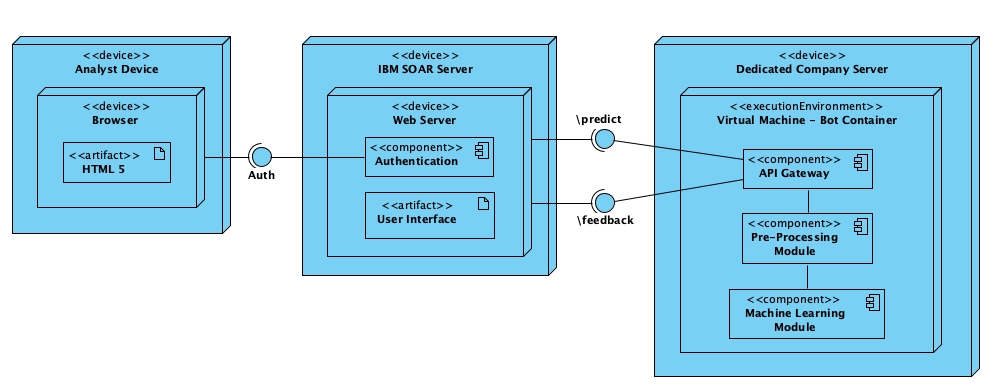
\includegraphics[width=\textwidth]{ch3/assets/archquiteture.png}
    \caption{Architecture of the Random Forest with Reinforcement Learning Feedback Loop Solution}
    \label{fig:architecture}
\end{figure}

It's organized into three major sections:
\begin{enumerate}
    \item \textbf{Analyst Device}: This device acts as the point of interaction where security analysts review and manage alerts. Represents the user interface. The analyst logs into the system through the \textbf{Authentication} component, enabling access to the dashboard.
    
    \item \textbf{IBM SOAR Server}: The IBM SOAR Server is the central system for managing security alerts. The server sends requests to the \textbf{Bot Container} through the \texttt{\textbackslash predict} endpoint, triggering the alert classification process. Once the alert is processed, the \texttt{\textbackslash feedback} endpoint is used to receive the analyst's input for further training of the RL model.
    
    \item \textbf{Dedicated Company Server}: The \textbf{Dedicated Company Server} hosts the \textbf{Bot Container}, which is deployed on a \textbf{Virtual Machine (VM)}. This container is responsible for the core functionality of the solution, consisting of three main components:
    \begin{itemize}
        \item \textbf{API Gateway}: This component serves as the entry point for receiving requests from the IBM SOAR Server and handling communication between the components inside the bot container. It processes the incoming alert data and forwards it to the appropriate modules.
        \item \textbf{Pre-Processing Module}: This module cleans and prepares the incoming alert data, extracting features and transforming them into a suitable format for the model.
        \item \textbf{Machine Learning Module}: The \textbf{Machine Learning Module} applies the \gls{RF} model to classify the alert. These predictions are then further refined through the \gls{RL} model.
    \end{itemize}
\end{enumerate}

This architecture is designed to be modular and scalable, allowing for easy integration with existing systems and the ability to adapt to evolving security threats.


%----------------------------------------------------------------------------------------

\subsection{Comparative Analysis}
Table~\ref{tab:solution_comparison} presents a comparison of the three proposed approaches based on key evaluation criteria. 
The goal is to assess their suitability in the context of a real-world SOC environment, taking into consideration implementation complexity, adaptability, performance, interpretability, and integration potential.

\captionsetup[table]{font=small} % Set the caption font size
\scriptsize % Reduce the font size for the table content
\begin{longtable}{@{}P{3cm}P{3cm}P{4cm}P{4cm}@{}}
    \caption{Comparison of Proposed Solutions}
    \label{tab:solution_comparison} \\
    \toprule
    \textbf{Criteria} & \textbf{\gls{RF} + \gls{RL}} & \textbf{\gls{DNN}} & \textbf{Rules + Decision Tree} \\
    \midrule
    \endfirsthead

    \toprule
    \textbf{Criteria} & \textbf{\gls{RF} + \gls{RL}} & \textbf{\gls{DNN}} & \textbf{Rules + Decision Tree} \\
    \midrule
    \endhead

    \bottomrule
    \endfoot

    \bottomrule
    \endlastfoot

    Architecture Type & \gls{RF} + \gls{RL} (Two-layer) & \gls{DNN} & Rule-based + Decision Tree \\
    \vspace{0.2cm}
    Implementation Complexity & Moderate & High & Low \\
    \vspace{0.2cm}
    Adaptability to New Threats & High (via \gls{RL}) & Moderate (via retraining) & Low (manual updates) \\
    \vspace{0.2cm}
    Learning from Feedback & Online (via \gls{RL}) & Periodic retraining & Batch/manual integration \\
    \vspace{0.2cm}
    Cold Start Handling & Excellent (\gls{RF} pre-trained) & Poor & Excellent (rules pre-set) \\
    \vspace{0.2cm}
    Interpretability & Moderate & Low & High \\
    \vspace{0.2cm}
    Scalability & High & High & Moderate \\
    \vspace{0.2cm}
    Integration with SIEM (IBM SOAR) & Easy & Easy & Easy \\
    \vspace{0.2cm}
    False Positive Reduction & Adaptive (confidence scoring) & Model confidence only & Rigid (rule-defined) \\
    \vspace{0.2cm}
    Performance in Evolving Scenarios & High & Moderate & Low \\
    
\end{longtable}

\normalsize

% \textbf{Solution 1} combines RF with RL, offering a highly adaptable system that continuously improves its performance over time. 
% The integration of RF for initial predictions and RL for feedback-based adjustments allows the system to react to evolving cybersecurity threats.

% \begin{itemize}
%     \item The implementation complexity is moderate, as integrating two models (RF and RL) requires careful setup but remains manageable with existing frameworks like scikit-learn and RLlib.
%     \item High adaptability, as the RL model continuously adjusts based on analyst feedback. The system can handle new attack patterns without requiring manual updates, making it effective in dynamic environments.
%     \item This solution uses online learning through the RL feedback loop, which means feedback from analysts is immediately integrated into the model, refining its predictions in real-time.
%     \item Excellent cold start handling, thanks to the pre-trained RF model. This allows the system to make predictions right away, with the RL model improving its performance gradually over time.
%     \item Moderate interpretability due to the transparency of the RF model, but the integration of RL adds complexity, making it harder to explain the decision-making process.
%     \item High performance in evolving scenarios, as the RL model adapts in real-time to new data, making it well-suited for fast-changing threat landscapes.
% \end{itemize}

% \textbf{Solution 2} uses a DNN that processes raw alert data through attention mechanisms to automatically extract features and classify alerts. 
% Unlike \textbf{Solution 1}, it doesn't use RL for real-time feedback but relies on periodic retraining to improve performance.

% \begin{itemize}
%     \item High implementation complexity because training a DNN requires substantial computational resources and time, especially when handling raw data with attention mechanisms. This makes it more complex to implement compared to \textbf{Solution 1}.
%     \item Moderate adaptability. The DNN model learns from feedback, but it does so through periodic retraining. It doesn't adjust in real-time like \textbf{Solution 1}, making it less responsive to new threats immediately after they emerge.
%     \item Feedback is applied during periodic retraining. This means the model improves over time but is slower to adapt compared to \textbf{Solution 1}, which has real-time learning through RL.
%     \item Poor cold start handling. The DNN model requires a significant amount of labeled data to be trained before it can start making reliable predictions. It cannot provide immediate predictions like \textbf{Solution 1}.
%     \item Low interpretability. DNN models are often considered “black boxes,” making it difficult to explain how certain predictions were made, especially when attention mechanisms are involved.
%     \item Moderate performance. While the DNN is effective on known data, it needs retraining to adjust to new, unseen patterns, making it less suited for dynamic cybersecurity environments compared to \textbf{Solution 1}.
% \end{itemize}

% \textbf{Solution 3} integrates static expert rules with a lightweight DTC. 
% The rule engine filters known patterns, while the DTC handles ambiguous or unknown cases. 
% Feedback is aggregated and applied periodically to retrain the decision tree and refine the rules.

% \begin{itemize}
%     \item Low implementation complexity. The system is built with simple decision tree algorithms and rule-based filtering, making it easier to implement compared to the more complex \textbf{Solution 1} and \textbf{Solution 2}.
%     \item Low adaptability. The system relies on manual updates to the rules base to address new attack vectors. It is not capable of real-time adjustments like \textbf{Solution 1}.
%     \item Feedback is applied asynchronously. The system doesn't adjust in real-time but instead uses periodic feedback to update the rules and retrain the decision tree. This makes it slower to improve and adapt to changing threats.
%     \item Excellent cold start handling. The rules-based system can immediately classify alerts based on predefined patterns, and the DTC can be deployed quickly without extensive data preparation.
%     \item High interpretability. Both the rule engine and DTC are transparent, allowing security analysts to easily understand the rationale behind decisions. This is a major advantage in environments that require auditing and explainability.
%     \item Low performance in evolving scenarios. The system relies on static rules, which require manual updates to accommodate new threats. It is less flexible than \textbf{Solution 1} or \textbf{Solution 2}, making it less effective in rapidly changing cybersecurity environments.
% \end{itemize}

% \subsubsection{Overall Evaluation}

Solution 1 is optimal because it offers adaptability, scalability, and real-time learning. 
Integrating RF with RL continuously adapts to new threats through real-time feedback, making it highly effective in dynamic cybersecurity environments.

Solution 2 excels in feature extraction using DNN but lacks immediate adaptability. 
It requires periodic retraining, making it less responsive to evolving threats than Solution 1.

Solution 3, while simple and interpretable, is not adaptable. 
It relies on static rules and manual updates, making it less suitable for fast-changing threat landscapes.

In conclusion, Solution 1 is the best option for real-time alert classification and long-term adaptability in a SOC environment.

\section{Proof of Concept}
This section presents the practical implementation of the proposed solution, including the setup of the test environment, preparation of the dataset, and execution of the ML models. It aims to demonstrate the feasibility and performance of the selected approach under realistic conditions.

\subsection{Data Processing}
This section outlines the process of refining the raw data, corresponding to phase B in the solution pipeline.

As previously mentioned, Solution One was the best choice among the three alternatives.

To implement this solution effectively, ArtResilia provided a dataset of security alerts generated by its SOC. 

This dataset, covering the period from February 9, 2022, to January 31, 2025, encompasses various alerts categorized by attributes, such as priority and taxonomy. 
The primary goal of the data processing phase was to prepare this raw data for training ML models to predict the priority and taxonomy of alerts based on the textual descriptions associated with each alert.

\begin{figure}[h!]
    \centering
    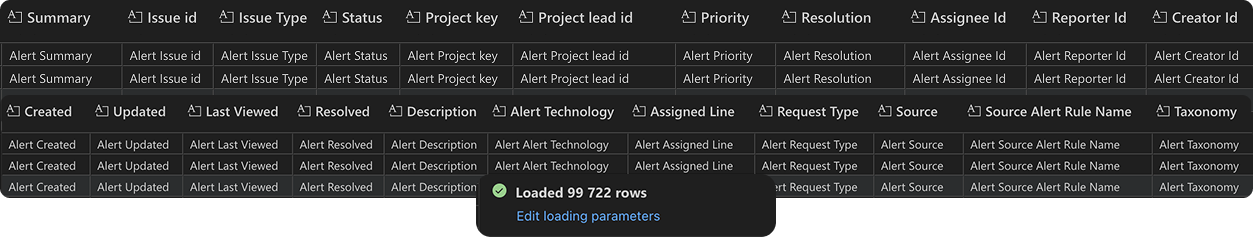
\includegraphics[width=\textwidth]{ch3/assets/dataset_original.png}
    \caption{Original Dataset Before Preprocessing}
    \label{fig:dataset_original}
\end{figure}

Figure~\ref{fig:dataset_original} illustrates the original dataset before preprocessing.
The dataset\footnote{For privacy reasons, the actual data has been censored or altered to ensure confidentiality.} contains 99,722 rows, each representing a security alert.

To prepare the data for training ML models, several key preprocessing steps were performed:

\paragraph{First Step}
Rows missing data in "Priority" or "Taxonomy" were removed, retaining only the essential columns: "Description", "Priority", and "Taxonomy". 
These columns provide the text for training and the target labels.

Listing~\ref{lst:first_preprocessing} shows the Python code snippet used for this initial preprocessing step.

\vspace{0.2cm}
\noindent
\begin{minipage}{\linewidth}
\begin{minted}{python}
df = df[(df['Source'] != 'Other') & (df['Source Alert Rule Name'].notna())]
required_columns = ["Description", "Priority", "Taxonomy"]
df = df[required_columns]
df = df.dropna(subset=required_columns)
\end{minted}
\captionof{listing}{Python Code Snippet for the First Part of Preprocessing the Dataset.}
\label{lst:first_preprocessing}
\end{minipage}
\vspace{0.1cm}

\paragraph{Second Step}
Alerts with a Priority of "P4" or a Taxonomy labeled as "Other" were also excluded as these were deemed less relevant for the model's prediction task. 
To address class imbalance in the Taxonomy column, random oversampling was performed. 
This involved ensuring that smaller categories had enough examples for the model by duplicating instances from underrepresented taxonomies until they matched the size of the largest category.

Listing~\ref{lst:second_preprocessing} provides the Python code snippet used for the second preprocessing step, which includes filtering and oversampling to address class imbalance in the dataset. 

\vspace{0.2cm}
\noindent
\begin{minipage}{\linewidth}
\begin{minted}{python}
df = df[(df["Priority"] != "P4") & (df["Taxonomy"].str.lower() != "other")]
taxonomy_counts = df["Taxonomy"].value_counts()
max_len = taxonomy_counts.max()
oversampled_dfs = []
for tax, count in taxonomy_counts.items():
    sub_df = df[df["Taxonomy"] == tax]
    if count < max_len:
        diff = max_len - count
        extra_rows = sub_df.sample(n=diff, replace=True, random_state=42)
        sub_df = pd.concat([sub_df, extra_rows], ignore_index=True)
    oversampled_dfs.append(sub_df)
df = pd.concat(oversampled_dfs, ignore_index=True)
\end{minted}
\captionof{listing}{Python Code Snippet for the Second Part of Preprocessing the Dataset.}
\label{lst:second_preprocessing}
\end{minipage}
\vspace{0.1cm}

By applying the preprocessing code above from steps one and two, the dataset was reduced from its original 99,722 rows, representing security alerts, to approximately 81,732 rows.
However, after the oversampling process, the dataset was expanded to around 173,637 rows, ensuring a balanced representation of all taxonomies.

\paragraph{Third Step}

The "Description" column, which contains raw text data, was also cleaned. 
Unnecessary formatting was removed as well as special characters, and irrelevant sections (such as URLs and IBM SOAR links). 
It also handled tasks like stripping extra whitespace and removing HTML tags, ensuring the text was in a consistent and usable format for the machine learning pipeline.

Listing~\ref{lst:third_preprocessing} shows the Python code snippet used for this third preprocessing step.

\vspace{0.2cm}
\noindent
\begin{minipage}{\linewidth}
\begin{minted}{python}
df["Description"] = df["Description"].progress_apply(clean_text)
\end{minted}
\captionof{listing}{Python Code Snippet for the Third Part of Preprocessing the Dataset.}
\label{lst:third_preprocessing}
\end{minipage}
\vspace{0.1cm}

The code snippet presented above applies the \texttt{clean\_text} function uniformly to all entries within the "Description" column of the dataset, ensuring consistent preprocessing of textual data for subsequent machine learning tasks.

The rules defined for normalizing the description text will be detailed in the next section, where the \texttt{clean\_text} function is explained.

\paragraph{Fourth Step}

Finally, the "Priority" and "Taxonomy" labels were stripped of any leading or trailing spaces to ensure consistency in the dataset. 

Listing~\ref{lst:fourth_preprocessing} shows the Python code snippet used for this final preprocessing step.

\vspace{0.2cm}
\noindent
\begin{minipage}{\linewidth}
\begin{minted}{python}
df["Priority"] = df["Priority"].astype(str).str.strip()
df["Taxonomy"] = df["Taxonomy"].astype(str).str.strip()
\end{minted}
\captionof{listing}{Python Code Snippet for the Fourth Part of Preprocessing the Dataset.}
\label{lst:fourth_preprocessing}
\end{minipage}
\vspace{0.1cm}

These preprocessing steps ensure that the dataset is clean, balanced, and properly formatted, making it ready for use in the ML models. 
The combination of filtering, oversampling, text cleaning, and label processing prepares the data for training while addressing potential issues such as class imbalance and noisy raw data.

\begin{figure}[h!]
    \centering
    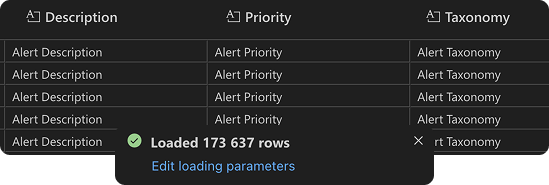
\includegraphics[width=\textwidth]{ch3/assets/dataset_processed.png}
    \caption{Original Dataset After Preprocessing}
    \label{fig:dataset_processed}
\end{figure}

Figure~\ref{fig:dataset_processed} illustrates the dataset\footnotemark[\value{footnote}] after preprocessing, showcasing the difference between the original and processed versions.

\subsection{Data Normalization}
Data normalization typically refers to the process of transforming data into a common scale to improve the performance and accuracy of machine learning models. 

In this project, normalization was applied specifically to the "Description" column, which contains the raw text data. 

This is crucial, as natural language data can contain noise, irrelevant characters, and inconsistencies that can negatively impact model training and performance. 

Unlike the Priority and Taxonomy columns, which are already in categorical formats suitable for ML models, the Description column required more extensive processing to make it usable for training.

As stated in the previous section, the normalization process was performed using a function called \texttt{clean\_text}, which was designed to normalize the raw text in the Description column. 
This function specifically targets common issues in textual data, such as extraneous formatting, unwanted characters, and irrelevant content.

\begin{figure}[h!]
    \centering
    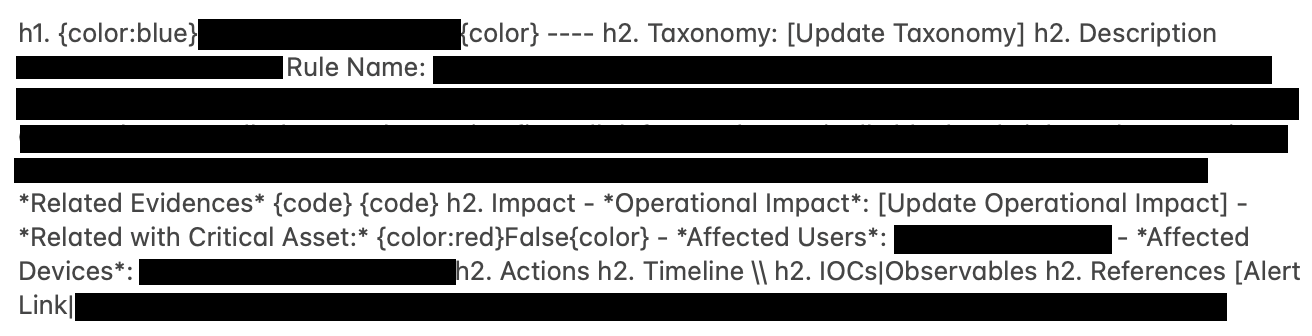
\includegraphics[width=\textwidth]{ch3/assets/redacted_description_text.png}
    \caption{Redacted Description Text}
    \label{fig:redacted_description_text}
\end{figure}

Figure~\ref{fig:redacted_description_text} presents a redacted\footnote{For privacy reasons, the actual data has been censored or altered to ensure confidentiality.} visualization that exemplifies the typical format of a description text.
The formatting of this description may differ based on the source of the alert, highlighting the diverse origins and structures of the data. 
To address these variations, the \texttt{clean\_text} function was created to standardize the presentation of the text data, ensuring it remains consistent regardless of its source.

The \texttt{clean\_text} function performs several key operations:

\begin{itemize}
    \item \textbf{Extract Relevant Content:} Identifies and retains the "Description" section, removing irrelevant sections like "Taxonomy" or "References" if present.
    \item \textbf{Remove Unwanted Characters:} Cleans special symbols, color tags, code markers, HTML tags, and URLs to retain only meaningful content.
    \item \textbf{Text Cleaning:} Strips extra spaces, removes irrelevant phrases (e.g., "action:" or "related evidences:"), and ensures consistent formatting.
    \item \textbf{Handle Rule Name:} Captures and formats rule names with associated narratives as \texttt{<Rule Name> - <Narrative>} for clarity.
    \item \textbf{Final Output:} Returns a cleaned, normalized description.
\end{itemize}

By applying a normalizing function to the Description column helps achieve consistency and reduce noise in the training text data.
The Priority and Taxonomy columns did not require the same normalization process, as they are categorical and do not need extensive text processing.

\subsection{Dataset Division}
Dataset Division refers to how the dataset is split into subsets used for training, validation, and testing. 

This division is crucial because it allows the model to be trained on one subset of the data while ensuring that the model's performance is evaluated on unseen data. 

This prevents overfitting, where the model performs well on training data but fails to generalize to new, unseen data. 

Similarly, proper dataset division also avoids underfitting, where the model might not learn enough from the training data to perform well.
\clearpage
In ML, the dataset is typically divided into three parts:
\begin{itemize}
    \item \textbf{Training Set:} Used to train the model.
    \item \textbf{Validation Set:} Used to tune the model's hyperparameters and prevent overfitting during training.
    \item \textbf{Test Set:} Used to evaluate the final model's performance after training is complete.
\end{itemize}

In this project, the dataset was divided as follows:

\begin{itemize}
    \item \textbf{Training and Test Split:} The data was split into 70\% for training and 30\% for testing. This ratio strikes a balance between providing enough data for the model to learn from, while still maintaining a sufficient amount of data to test its generalization ability. This approach was chosen to maximize the model's ability to generalize to unseen data while preventing overfitting.
\end{itemize}

\vspace{0.2cm}
\noindent
\begin{minipage}{\linewidth}
\begin{minted}{python}
X_train, X_test, Y_train, Y_test = train_test_split(X, Y, test_size=0.3, random_state=42, stratify=stratify_labels)
\end{minted}
\captionof{listing}{Splitting Dataset.}
\label{lst:dataset_split}
\end{minipage}
\vspace{0.1cm}

\begin{itemize}
    \item \textbf{Stratified Sampling:} The split was performed using stratified sampling, ensuring that the proportion of each class in Priority and Taxonomy was maintained across the training and test sets. This helps avoid bias in the dataset and ensures that both the training and test sets have representative distributions of all classes.
\end{itemize}

\vspace{0.2cm}
\noindent
\begin{minipage}{\linewidth}
\begin{minted}{python}
stratify_labels = [tuple(row) for row in Y]
X_train, X_test, Y_train, Y_test = train_test_split(X, Y, test_size=0.3, random_state=42, stratify=stratify_labels)
\end{minted}
\captionof{listing}{Stratified Sampling.}
\label{lst:stratified_sampling}
\end{minipage}
\vspace{0.1cm}

This stratified split is particularly important for imbalanced datasets, as it ensures that each class is proportionally represented in both the training and testing subsets, thereby improving the model's ability to generalize and minimizing bias toward the majority class.

\begin{itemize}
    \item \textbf{Test Set}: The 30\% test set was kept completely separate from the training process, ensuring that the model's performance could be assessed on data it had never seen before. This provides an unbiased evaluation of the model's accuracy and generalization capabilities.
\end{itemize}

By properly dividing the dataset, this approach ensures that the model is trained on a representative subset of data, can be fine-tuned using the validation set, and is evaluated fairly on the test set. 
This helps in achieving a balance between training the model effectively and ensuring generalization without overfitting or underfitting.

\subsection{Machine Learning Model Development}
In this section, the implementation of selected machine learning algorithms is discussed.

\subsection{Hyperparameter Tuning}
Details of the strategy used to tune hyperparameters and optimize the models' performance.
